\documentclass{beamer}
\usepackage{listings}
\lstset{
%language=C,
frame=single, 
breaklines=true,
columns=fullflexible
}
\usepackage{subcaption}
\usepackage{url}
\usepackage{tikz}
\usepackage{tkz-euclide} % loads  TikZ and tkz-base
%\usetkzobj{all}
\usetikzlibrary{calc,math}
\usepackage{float}
\newcommand\norm[1]{\left\lVert#1\right\rVert}
\newcommand{\Lagr}{\mathcal{L}}
\renewcommand{\vec}[1]{\mathbf{#1}}
\providecommand{\pr}[1]{\ensuremath{\Pr\left(#1\right)}}
\usepackage[export]{adjustbox}
\usepackage[utf8]{inputenc}
\usepackage{amsmath}
\usetheme{Madrid}

\title{Research Paper - Presentation}
\author{G Vojeswitha  - AI20BTECH11024}

\begin{document}
\begin{frame}
\titlepage
\end{frame}
\section{Title and Authors}
\begin{frame}
\frametitle{Title and Authors}
\begin{block}{Title}
OBS network blocking probability prediction using ensemble technique 
\end{block}
\begin{block}{Authors}
\begin{enumerate}
    \item Srija Chakraborty, Dept. of C.S.E.,National Institute of Technology, Rourkela, India, 518CS6016@nitrkl.ac.in
    \item Ashok Kumar Turuk, Dept. of C.S.E.,National Institute of Technology, Rourkela, India, akturuk@nitrkl.ac.in
    \item Bibhudatta Sahoo, Dept. of C.S.E., National Institute of Technology, Rourkela, India, bdsahu@nitrkl.ac.in
\end{enumerate}
\end{block}
\end{frame}

\section{\textbf{Introduction}}
\subsection*{OBS network}
\begin{frame}[fragile]
\frametitle{OBS Networking and Blocking Probability}
 \begin{enumerate}
    \item \textbf{Optical Burst Switching Networks(OBS NETWORK)}: \\It is a optical networking technique that allows sub-wavelength switching of data. Among other existing switching techniques, OBS performs better for network with high traffic. 
    \item \textbf{Data Burst Packet - }The packet containing the data to be transmitted.
    \item \textbf{Burst Control Packet(BCP) -} A control signal containing all the routing instructions of data burst. BCP is transmitted prior to data burst.
    \item Burst contention occurs
whenever at the time of transmission burst gets blocked. If the blocking probability can be predicted for a network, then the performance of the network can be improved
    \item The \textbf{Blocking probability} of any network can be determined by calculating the proportion of the count of the bursts (lost) divided by the aggregate count of burst (sent).
\end{enumerate}
\end{frame}

\subsection*{Abstract}
\begin{frame}[fragile]
\frametitle{Abstract}
\begin{block}{}
   \begin{enumerate}
\item . In the proposed technique, different predictor models and feature reduction algorithms are used to predict the blocking probability of upcoming traffic in a OBS network which will help us improve the performance of the
network drastically
\item The proposed model is able to predict the blocking probability with higher accuracy, along with lowering the number of burst loss by wavelength conversion strategy. Thus, it will help future network designers to have an
advanced idea about the performance of the network under specific framework.
\item Any Eventdriven simulator can be used to calculate the blocking probability simulation. Erlang fixed point approximation(EFPA) is used for analytical approach. However, these traditional approaches are much more time-consuming and tedious. Therefore, different AI techniques are used for prediction.
\end{enumerate}
\end{block}
\end{frame}

\begin{frame}[fragile]
\frametitle{Proposed architecture of this approach}
\begin{figure}
    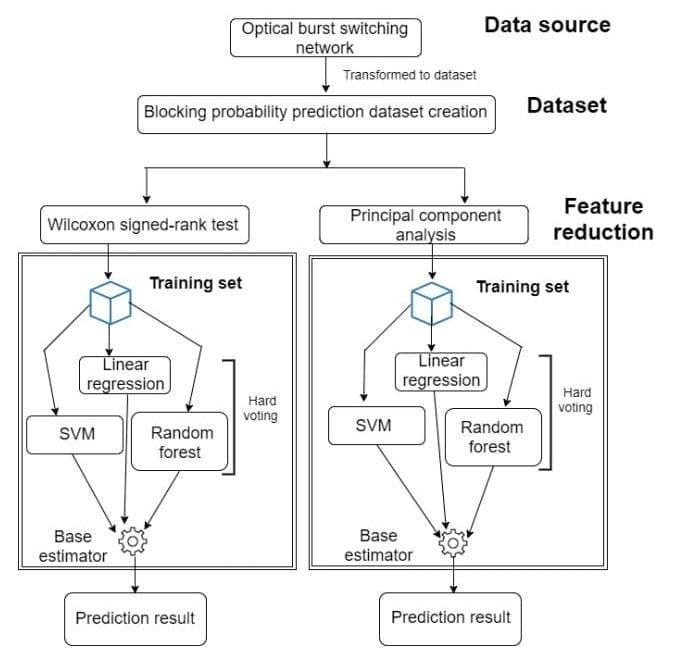
\includegraphics[scale=0.33]{proposed approach.jpeg}
\end{figure}
\end{frame}

\section{\textbf{Proposed technique}}
\subsection*{Data Set Creation}
\begin{frame}[fragile]
\frametitle{Dataset creation}
\begin{block}{}
   Seven independent input parameters are taken as input. With help of these input parameters, proposed ensemble model is trained to study the mapping from the condition of the network and predict the blocking probability.
  \begin{table}[ht]
  \centering
  \begin{tabular}{|c|c|}
        \hline
         E & Mean traffic load in S-D pair\\
         \hline
         D & Diff b/w max, min traffic load\\ \hline
         C & Number of channels per wavelength \\
        \hline
         W & Number of wavelengths \\
        \hline
         \(T_{off}\) & Offset time\\
        \hline
        APL & Average path length\\
        \hline
        CR  & Concentration of rout \\ 
        \hline
    \end{tabular}
    \caption{}
\end{table}
\end{block}
 \end{frame}

\subsection*{Feature reduction}
\begin{frame}[fragile]
\frametitle{Feature reduction techniques}
\begin{block}{}
    \begin{enumerate}
     \item For faster prediction, dimensionality of large data sets are reduced, by transforming a large set of variables into a smaller set that still contains most of the information in the large set.
     \item Reducing the number of variables of a data set naturally comes at the expense of accuracy,but smaller data sets are easier to explore and visualize and make analyzing data much easier and faster for machine learning algorithms.
     \item In this proposed model, Wilcoxon signed-rank test and Principal component analysis (PCB) are the feature reduction techniques used to remove least important features.
\end{enumerate}
\end{block}
\end{frame}

\begin{frame}[fragile]
\frametitle{Wilcoxon Signed Rank Test}

\begin{block}{}
   \begin{enumerate}
   %\item This technique is used for the analysis of matched pair data. 
    \item The null hypothesis of this test is 'probability distribution of set of pair wise differences is centered at 0'.For this procedure, differences comes from a continuous distribution  
    \item Test statistics for this procedure are calculated by either adding the ranks assigned to the positive differences \(T_{+}\) or by adding the ranks assigned to the negative differences \(T_{-}\).
    \begin{align}
        T_{+} + T_{-} = \frac{n(n+1)}{2}
    \end{align}
    where n = no.of samples of the data.
\end{enumerate}
\end{block}
    
\end{frame}

\begin{frame}[fragile]
\frametitle{Wilcoxon Signed Rank Test (contd)}
\begin{block}{}
   \begin{enumerate}
    \item However for large samples, Z is used as standard normal distribution to test the hypothesis.
    \begin{align}
        Z^{+}= \dfrac{\frac{T^{+}-n(n+1)}{4}}{\left\{\frac{n(n+1)(2n+1)}{24}\right\}^{\frac{1}{2}}}
    \end{align}
    \item  Null hypothesis is analysed by forming a rejection region for test statistic \(T_{+}\) or \(T_{-}\). 
    \\A two-tailed rejection region for the null
    hypothesis based on \(T_{+}\) is used.
\end{enumerate}
\end{block}
\end{frame}

\begin{frame}[fragile]
\frametitle{Principal Component Analysis}
\begin{block}{}
   It is a technique used to convert a set of possibly co-related variables to that of linearly uncorrelated variables using orthogonal transformation. Using eigen values and eigen vectors, data is categorised based on their similarities and differences.\\
The following equation is used to achieve the decreased dimensional data
\begin{align}
    Y = Z^T X
\end{align}
where $Y = $ Final Data Set, $X=$ Original Data Set, Z is the orthogonal matrix containing eight eigen vectors.
\end{block}
\end{frame}

\begin{frame}[fragile]
\frametitle{Wilcoxon Signed Rank Test vs PCA}
   \begin{block}{}
       For a dataset of OBS network, PCA reduced more unwanted features than wilcoxon signed-rank test.
    \end{block}
\end{frame}

\subsection*{Predictor Techniques}
\begin{frame}[fragile]
\frametitle{Predictor techniques}
\begin{enumerate}
    \item In this work, ensemble of predictors like
Linear Support Vector Machine (SVM), Linear Regression (LR)
and Random Forest (RF) are used to train and predict burst
contention or burst blocking probability
\item  To acomplish
ensemble, we use bagging and as we predict the exact result instead of probable result, we use hard voting. In our model,
hybridization is done by bagging.
\item In bagging, we use same predictor many times and the
training instances are sampled.
\item After using each model, we will get accuracy for each
of them. Using each of these results, we can make a better
prediction by aggregating the predicted results and by voting
for the final class, which has more number of votes

\end{enumerate}
\end{frame}

\begin{frame}[fragile]
\frametitle{Linear Support Vector Machine}
\begin{block}{}
   \begin{enumerate}
    \item  \(w^{T}\)x is the hyperplane of linear SVMs which segregate
    data points of two classes optimally
\\Here w is a hyperplane that learns from data using SGD (stochastic gradient descent).
\item In this algorithm, the
objective function E(w) used in SGD as a feature vector,
\begin{align}
    E(w) = \frac{1}{p}  \sum_{i=1}^{p} L(y_{i},w^{T}x_{i}) + a||w||^2
\end{align}
where \( x_{i}\) \(\in\) X and respectively \(y_{i}\) lies between 0 to 1

\\a is regularisation constant \\
and L is the loss function defined as 
\begin{align}
    L(t,y) = max(0, 1-t(y))
\end{align}
\end{enumerate}
\end{block}
\end{frame}

\begin{frame}[fragile]
\frametitle{Linear regression}
\begin{block}{}
   \begin{enumerate}
  \item Equation of this model : Y = aX + b 
 \\where X is the independent variable, a is the slope and b is the y-intercept. Here a and b can be calculated using equation 5 and 6.
 \begin{align}
     a = \frac{(\sum y)(\sum x^{2}) - (\sum x)(\sum xy) }{n.(\sum x^{2}) - (\sum x)^{2}}
 \end{align}
 \begin{align}
      b = \frac{n(\sum xy) - (\sum x)(\sum y) }{n.(\sum x^{2}) - (\sum x)^{2}}
 \end{align}
\end{enumerate}
\end{block}
\end{frame}

\begin{frame}[fragile]
\frametitle{Random Forest}
\begin{block}{}
   \begin{enumerate}
    \item  In this algorithm, best features are not searched while splitting a node rather than it is searched among a random subset of features.
    \item The classification formula for this model is:
\begin{align}
    J(k,t_{k}) = \frac{m_{left}}{m}G_{left} + \frac{m_{right}}{m}G_{right} 
\end{align}
Where G evaluates the impurity of the subsets left and right and m represents the total number of instances available in the subsets.
\end{enumerate}
\end{block}
\end{frame}

\begin{frame}[fragile]
\frametitle{Training model}
\begin{enumerate}
    \item   Random forest is prefered to
     use since it works efficiently on large dataset while SVM and linear regression are weak learners.
     \item After training is performed utilizing the linear regression, next we train the model using a linear support vector machine.At the last stage of algorithm, random forest algorithm is used.
    \item With linear regression, the samples can be predicted with higher or lower accuracy.
    \item Linear SVMs work efficiently most of the times, many datasets are not even being linearly separable. For getting that situation to regularise the SVM, we have set C=1 and loss hyperparameter to “hinge”
\end{enumerate}
\end{frame}

\begin{frame}[fragile]
\frametitle{Training model(contd)}
\begin{enumerate}
    \item The parameters which are used in random forest are the maximum depth of tree, random state and also the minimum number of samples needed for splitting an internal node and the minimum number of samples needed to be at a leaf node.
    \item All the selected samples should be considered at the time of splitting the internal node.
    In a tree, if it leaves at least minimum training samples in each of the left and right branches, then it is considered as a split point at any depth.

\end{enumerate}
\end{frame}


\begin{frame}[fragile]
\frametitle{Algorithmn: Blocking probability prediction model}
\begin{figure}
    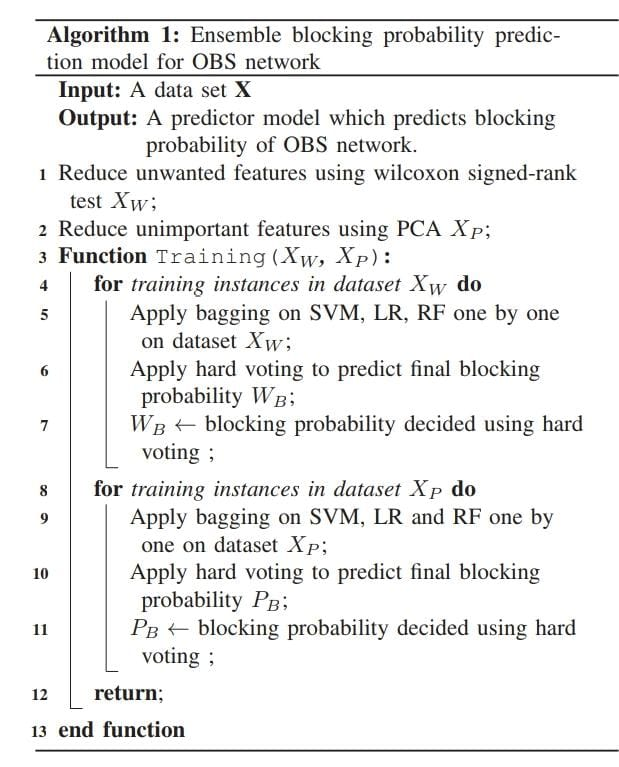
\includegraphics[scale=0.30]{algorithm.jpeg}
\end{figure}
\end{frame}

  
\begin{frame}[fragile]
\frametitle{Experiment results}
\begin{figure}
    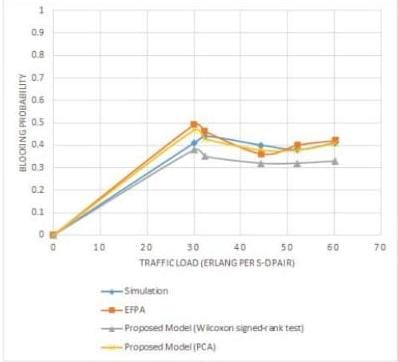
\includegraphics[scale=0.48]{exp_1.jpeg}
    \caption{Blocking probability estimation by Simulation, EFPA, proposed ensemble model with wilcoxon signed-rank test and proposed ensemble model with PCA with setting D = 6, C= 40, W= 3, Toff = 0.0000086, APL= 3.75, CR= 3}
\end{figure}
\end{frame}

\begin{frame}[fragile]
\frametitle{Experiment results}
\begin{figure}
    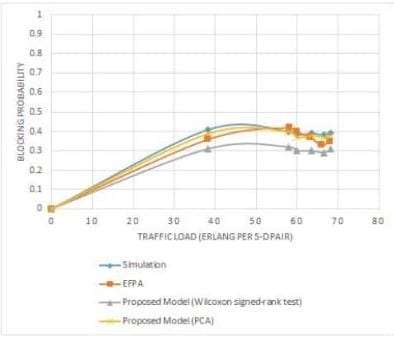
\includegraphics[scale=0.48]{exp_2.jpeg}
    \caption{ Blocking probability estimation by ensemble proposed model, ADMM-I-ELM, ADMM-Log-I-ELM, EFPA, Simulation with setting D=10, C=18, W=5, Toff = 0.000009, APL=2.628, CR=2.25}
\end{figure}
\end{frame}


\begin{frame}[fragile]
\frametitle{Experiment results}
\begin{block}{}
\begin{enumerate}
       \item While applying ensemble with wilcoxon
signed-rank test technique as feature reduction, the root-mean square error(RMSE) is calculated as \(7.4 \times 10^{-4}\) and with  PCA technique as feature reduction, the root-meansquare error(RMSE) is calculated as \(2.3 \times 10^{-4}\)
\item  The first feature reduction technique used is wilcoxon signed-rank test which does not perform well for this model and gives only 80 \% accuracy
\item However, for the second technique which is principal component analysis, it performs
much better and gives 97 \% accuracy for the dataset obtained from OBS network
   \end{enumerate}
   \end{block}
   
\end{frame}

\end{document}